%%%%%%%%%%%%%%%%%%%% chapter.tex %%%%%%%%%%%%%%%%%%%%%%%%%%%%%%%%%%
% Chapter 10: Optical & Wireless Networks-on-Chip (ONoC / WNoC)
% Springer Nature Monograph svmono format
%%%%%%%%%%%%%%%%%%%%%%%%%%%%%%%%%%%%%%%%%%%%%%%%%%%%%%%%%%%%%%%%%%%

\chapter{Optical \& Wireless Networks-on-Chip (ONoC / WNoC)}
\label{chap:optical-wireless}

\abstract*{As many-core processors scale to hundreds of compute tiles, traditional electrical copper interconnects encounter severe physical throughput and energy barriers governed by wire aspect ratios, capacitive charging delays, and dielectric losses. To overcome these metallic wire limits, two disruptive non-traditional interconnect paradigms have emerged: Optical Networks-on-Chip (ONoC) utilizing silicon nanophotonics, and Wireless Networks-on-Chip (WNoC) utilizing on-chip millimeter-wave (mmWave) and sub-terahertz (sub-THz) electromagnetic radiation. ONoCs exploit silicon waveguides, Wavelength Division Multiplexing (WDM), and electro-optic Micro-Ring Resonators (MRRs) to route data at the speed of light with data-rate-independent transmission energy. Concurrently, WNoCs leverage integrated planar antennas and On-Off Keying (OOK) transceivers to provide single-cycle, low-latency global broadcast channels that bypass multi-hop router traversals. However, optical and wireless fabrics face acute physical implementation challenges: ONoCs suffer from waveguide crossing losses, modal crosstalk, and severe thermal resonance drifts ($\approx 0.1\,\mathrm{nm/^\circ C}$), while WNoCs are constrained by lossy silicon substrates, antenna footprint scaling, and power amplifier energy dissipation. This chapter provides a rigorous physical, architectural, and analytical treatment of optical and wireless on-chip networks. We model optical waveguide losses, contrast Crossing Switching Elements (CSEs) against Parallel Switching Elements (PSEs) based on Kao et al. (IEEE TCAD 2026), formulate system-level thermal resonance tracking based on Ye et al. (IEEE TVLSI 2013), and analyze channel-aware mmWave transceiver link budgets based on Shahmoradi et al. (IEEE TCAS-I 2026), complete with cycle-accurate optical loss simulation models and synthesizable Verilog photonic switch controllers.}

\section{The Non-Traditional Interconnect Paradigm}
\label{sec:optical-wireless-intro}

\begin{svgraybox}
\textbf{High-School Intuition: Garden Hoses vs. Laser Pointers} \\
Why replace copper wires with light beams and wireless radio waves?
\begin{itemize}
    \item \textbf{The Copper Wire (The Garden Hose)}: To get water out of a long empty garden hose, you first have to fill up the entire volume of the hose under pressure. In microchips, every copper wire has electrical capacitance ($C$); before a signal arrives, the transmitter must spend electrical energy charging the entire wire, generating latency and heat.
    \item \textbf{The Optical Waveguide (The Laser Pointer)}: Shining a laser pointer across the room delivers photons instantly at the speed of light ($85{,}000\,\mathrm{km/s}$ in silicon). Once turned on, it takes zero extra energy whether you blink it slowly or billions of times per second!
    \item \textbf{The Wireless Link (The Walkie-Talkie)}: Passing packets across a 64-core grid of routers is like whispering a message down 14 rows of desks in a classroom. A wireless link is like speaking into a walkie-talkie: every core in the room hears the broadcast in a single clock cycle!
\end{itemize}
\end{svgraybox}

In conventional electrical Networks-on-Chip, global packet delivery across large silicon dies requires multi-hop store-and-forward or wormhole router hops. Each intermediate hop incurs input buffering, arbitration latency, and crossbar traversal energy, while long copper wire segments dissipate substantial dynamic power ($P \propto \alpha C V^2 f$). 

Optical and wireless interconnects represent complementary physical solutions to the on-chip communication crisis:

\begin{enumerate}
    \item \textbf{Optical Interconnects (Lightwaves)}: Photons travel through silicon waveguides at the phase velocity of light in silicon ($v = c / n_{\mathrm{Si}} \approx 8.5 \times 10^7\,\mathrm{m/s}$). Unlike electrons in metallic wires, optical signals experience negligible data-dependent transmission energy; once an optical carrier is generated and modulated, photon propagation along a passive silicon waveguide dissipates minimal power regardless of bit rate. Furthermore, Wavelength Division Multiplexing (WDM) enables dozens of independent concurrent channels to share a single physical waveguide.
    
    \item \textbf{Wireless Interconnects (Electromagnetic Waves)}: On-chip wireless links transmit radio-frequency (RF) electromagnetic waves through integrated planar antennas at frequencies ranging from $28\,\mathrm{GHz}$ to $245\,\mathrm{GHz}$. Wireless links bypass the multi-hop diameter of planar meshes, delivering single-hop broadcast capabilities that accelerate cache coherence invalidations, synchronization barriers, and deep learning reduction collectives.
\end{enumerate}

\section{Silicon Nanophotonics Physical Foundations}
\label{sec:nanophotonics-foundations}

\begin{svgraybox}
\textbf{High-School Intuition: The Optical Tuning Fork} \\
A musical tuning fork vibrates only when a sound matches its exact pitch. A \textbf{Micro-Ring Resonator (MRR)} is an optical tuning fork: it captures only one specific color (wavelength $\lambda_{\mathrm{res}}$) of light while letting all other colors pass straight through. This allows \textbf{Wavelength Division Multiplexing (WDM)}: sending 16 to 64 independent colors of light down a single microscopic silicon tube simultaneously!
\end{svgraybox}

Silicon nanophotonics leverages standard CMOS silicon-on-insulator (SOI) fabrication processes. An active silicon core layer ($n_{\mathrm{Si}} \approx 3.48$) is encapsulated by a silicon dioxide cladding layer ($\mathrm{SiO_2}$, $n_{\mathrm{ox}} \approx 1.45$). The large refractive index contrast ($\Delta n \approx 2.03$) provides strong optical confinement via Total Internal Reflection (TIR), enabling microscopic sub-micron waveguide cross-sections (typically $450\text{--}500\,\mathrm{nm}$ wide by $220\,\mathrm{nm}$ high) with bend radii as tight as $3\text{--}5\,\mu\mathrm{m}$.

\subsection{Micro-Ring Resonators (MRRs)}

The fundamental building block of optical routing is the \textbf{Micro-Ring Resonator (MRR)}. An MRR consists of a circular looped optical waveguide positioned in close proximity to one or two straight bus waveguides. When light traveling along the bus waveguide satisfies the constructive interference resonant condition:
\begin{equation}
    m \lambda_{\mathrm{res}} = 2 \pi R \cdot n_{\mathrm{eff}}
    \label{eq:mrr-resonance}
\end{equation}
where $m \in \mathbb{N}$ is the azimuthal mode order, $R$ is the ring radius, and $n_{\mathrm{eff}}$ is the effective refractive index, optical energy couples evanescently into the ring cavity. Resonant wavelengths are diverted into the drop port, while non-resonant optical wavelengths pass unobstructed through the through port.

\subsection{Switching Element Architectures: CSE vs. PSE}

As analyzed by Kao et al.~\cite{Kao2026} and illustrated in Fig.~\ref{fig:kao-mrr-structures}, optical switching elements are classified into two structural topologies:

\begin{figure}[htbp]
\centering
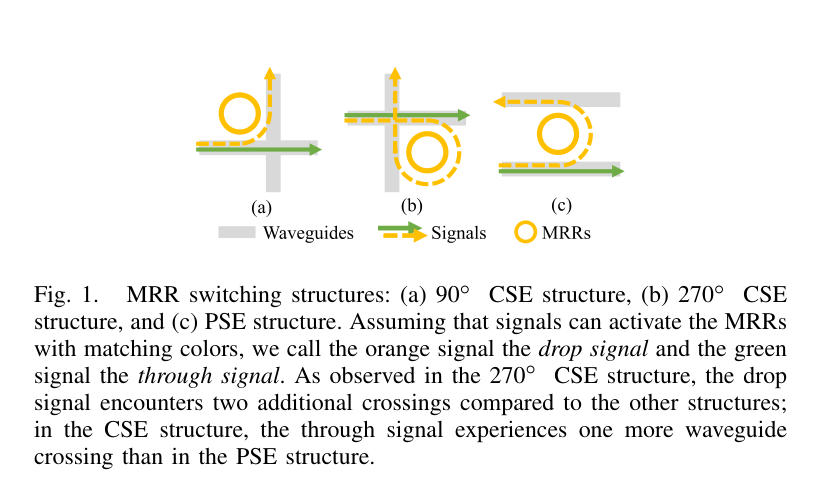
\includegraphics[width=0.88\textwidth]{chapters/ch10-optical-wireless/figures/kao_fig01_mrr_structures.png}
\caption{Micro-Ring Resonator (MRR) switching element structures: (a) $90^\circ$ Crossing Switching Element (CSE), (b) $270^\circ$ CSE, and (c) Parallel Switching Element (PSE). [Reproduced from: W.-Y. Kao et al., ``Provably Good Physically Aware WRONoC Design for Customized and Fault-Tolerant Topologies With Parallel Switching Elements and Sequence-Based Models'', \emph{IEEE Transactions on Computer-Aided Design of Integrated Circuits and Systems}, Vol. 45, No. 3, pp. 650--663, 2026, DOI: 10.1145/3658617.3697557.~\cite{Kao2026} \copyright\ 2026 IEEE]}
\label{fig:kao-mrr-structures}
\end{figure}

\begin{enumerate}
    \item \textbf{Crossing Switching Elements (CSEs)}: In CSE structures (Fig.~\ref{fig:kao-mrr-structures}(a) and (b)), the MRR is placed adjacent to an orthogonal waveguide crossing. While CSEs naturally align with traditional Manhattan orthogonal grid layouts, every waveguide crossing introduces insertion loss ($0.1\text{--}0.2\,\mathrm{dB}$) and inter-channel crosstalk noise. When signals drop through a CSE, they encounter additional waveguide crossings, amplifying worst-case optical losses.
    
    \item \textbf{Parallel Switching Elements (PSEs)}: In PSE structures (Fig.~\ref{fig:kao-mrr-structures}(c)), the MRR is positioned between two parallel waveguides. PSEs eliminate internal waveguide crossings entirely. When coupled with Add-Drop Filters (ADFs), as shown in Fig.~\ref{fig:kao-adf-structures}, PSE structures provide $2\times 2$ spatial switching without crossing penalties.
\end{enumerate}

\begin{figure}[htbp]
\centering
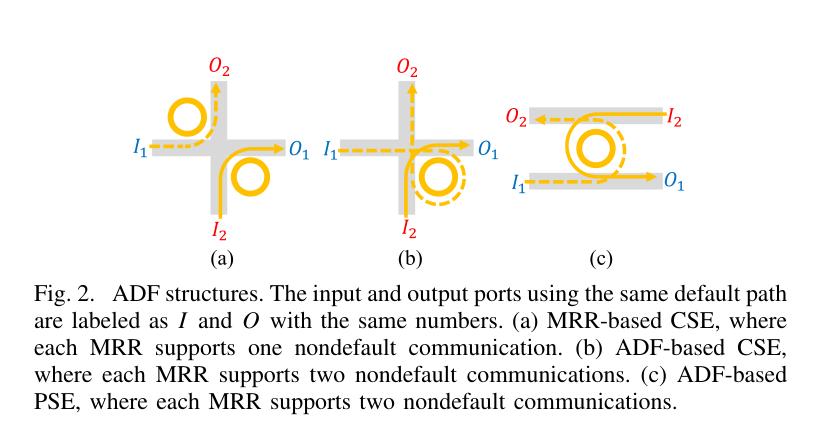
\includegraphics[width=0.88\textwidth]{chapters/ch10-optical-wireless/figures/kao_fig02_adf_structures.png}
\caption{Add-Drop Filter (ADF) structures with default paths (straight through) and non-default paths (dropped via MRR coupling). [Reproduced from: W.-Y. Kao et al., ``Provably Good Physically Aware WRONoC Design for Customized and Fault-Tolerant Topologies With Parallel Switching Elements and Sequence-Based Models'', \emph{IEEE Transactions on Computer-Aided Design of Integrated Circuits and Systems}, Vol. 45, No. 3, pp. 650--663, 2026, DOI: 10.1145/3658617.3697557.~\cite{Kao2026} \copyright\ 2026 IEEE]}
\label{fig:kao-adf-structures}
\end{figure}

\section{Optical Loss Modeling, Link Budgets \& Laser Power}
\label{sec:optical-loss-budget}

\subsection{Component Insertion Loss Decomposition}

An optical signal propagating from a Continuous-Wave (CW) laser source, through a modulator, across the routing network, and into a Germanium photodetector accumulates optical insertion losses along its path:
\begin{equation}
    L_{\mathrm{path}}(\mathrm{dB}) = L_{\mathrm{prop}} + L_{\mathrm{bend}} + L_{\mathrm{cross}} + L_{\mathrm{thru}} + L_{\mathrm{drop}} + L_{\mathrm{mod}}
    \label{eq:optical-loss-sum}
\end{equation}
where:
\begin{itemize}
    \item $L_{\mathrm{prop}} = \alpha_{\mathrm{prop}} \cdot l_{\mathrm{wg}}$ represents optical scattering propagation loss along waveguide length $l_{\mathrm{wg}}$ (typically $\alpha_{\mathrm{prop}} \approx 0.2\text{--}0.5\,\mathrm{dB/cm}$).
    \item $L_{\mathrm{bend}} = N_{\mathrm{bend}} \cdot \alpha_{\mathrm{bend}}$ represents radiation losses from waveguide bends ($\approx 0.005\,\mathrm{dB/bend}$).
    \item $L_{\mathrm{cross}} = N_{\mathrm{cross}} \cdot \alpha_{\mathrm{cross}}$ represents crossing attenuation ($\approx 0.10\text{--}0.15\,\mathrm{dB/crossing}$).
    \item $L_{\mathrm{thru}} = N_{\mathrm{thru}} \cdot \alpha_{\mathrm{thru}}$ represents off-resonance transmission loss through unselected MRRs ($\approx 0.01\text{--}0.02\,\mathrm{dB/MRR}$).
    \item $L_{\mathrm{drop}} = N_{\mathrm{drop}} \cdot \alpha_{\mathrm{drop}}$ represents on-resonance drop coupling loss ($\approx 0.5\text{--}1.0\,\mathrm{dB/drop}$).
    \item $L_{\mathrm{mod}}$ is the electro-optic modulator insertion loss ($1.0\text{--}2.0\,\mathrm{dB}$).
\end{itemize}

\subsection{Laser Power Scaling \& Wall-Plug Efficiency}

To guarantee a Bit Error Rate (BER) $\le 10^{-12}$, the received optical power $P_{\mathrm{rx}}$ must exceed the photodetector receiver sensitivity $P_{\mathrm{sens}}$ (typically $-18\text{ to }-22\,\mathrm{dBm}$). The required optical output power of the CW laser source is governed by the worst-case path loss ($L_{\mathrm{max}}$):
\begin{equation}
    P_{\mathrm{laser\_opt}}(\mathrm{dBm}) = P_{\mathrm{sens}}(\mathrm{dBm}) + L_{\mathrm{max}}(\mathrm{dB}) + M_{\mathrm{margin}}(\mathrm{dB})
    \label{eq:laser-opt-power}
\end{equation}
where $M_{\mathrm{margin}} \approx 3\,\mathrm{dB}$ is an optical link operating margin. Converting to electrical power requires accounting for the Wall-Plug Efficiency ($\eta_{\mathrm{wpe}} \approx 15\text{--}25\%$) of off-chip or co-packaged Distributed Feedback (DFB) lasers:
\begin{equation}
    P_{\mathrm{laser\_elec}} = \frac{10^{(P_{\mathrm{laser\_opt}} / 10)}}{\eta_{\mathrm{wpe}}} \quad (\mathrm{mW})
    \label{eq:laser-elec-power}
\end{equation}
Because laser power scales exponentially with insertion loss in decibels ($P \propto 10^{L_{\mathrm{max}}/10}$), reducing worst-case optical losses by even $3\,\mathrm{dB}$ halves the entire laser electrical power dissipation.

\section{Thermal Sensitivity \& Closed-Loop Resonance Tuning}
\label{sec:optical-thermal-effects}

\begin{svgraybox}
\textbf{High-School Intuition: The Out-of-Tune Guitar} \\
If you leave a guitar in the hot sun, the wooden neck and metal strings expand, throwing the instrument completely out of tune! Silicon does the exact same thing: when a multi-core processor runs hot, silicon's refractive index rises ($dn_{\mathrm{Si}}/dT$), expanding the optical cavity and drifting resonant wavelengths by $\approx 0.10\,\mathrm{nm/^\circ C}$. To prevent data channels from detuning, tiny integrated electric microheaters warm cooler resonators to a steady baseline temperature.
\end{svgraybox}

\begin{figure}[htbp]
\centering
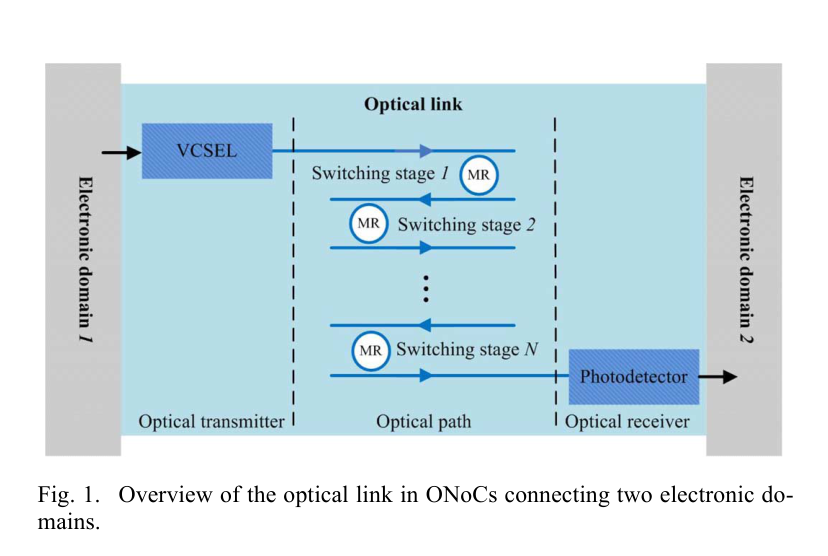
\includegraphics[width=0.88\textwidth]{chapters/ch10-optical-wireless/figures/ye_fig01_onoc_thermal_drift.png}
\caption{System-level thermal simulation of an Optical NoC demonstrating core active power dissipation, non-uniform on-chip temperature distributions, and resonant wavelength shifts in micro-ring resonators. [Reproduced from: Y. Ye et al., ``System-Level Modeling and Analysis of Thermal Effects in Optical Networks-on-Chip'', \emph{IEEE Transactions on Very Large Scale Integration (VLSI) Systems}, Vol. 21, No. 2, pp. 292--305, 2013, DOI: 10.1109/TVLSI.2012.2185524.~\cite{Ye2013} \copyright\ 2013 IEEE]}
\label{fig:ye-thermal-drift}
\end{figure}

Silicon exhibits a large positive thermo-optic coefficient:
\begin{equation}
    \frac{dn_{\mathrm{Si}}}{dT} \approx 1.86 \times 10^{-4}\,\mathrm{K^{-1}}
    \label{eq:thermo-optic-coeff}
\end{equation}
As modeled by Ye et al.~\cite{Ye2013} and depicted in Fig.~\ref{fig:ye-thermal-drift}, localized processor temperature fluctuations shift the effective refractive index of the silicon cavity, causing the MRR resonant wavelength to drift:
\begin{equation}
    \frac{d\lambda_{\mathrm{res}}}{dT} = \frac{\lambda_{\mathrm{res}}}{n_{\mathrm{g}}} \frac{dn_{\mathrm{Si}}}{dT} \approx 0.08\text{--}0.11\,\mathrm{nm/^\circ C}
    \label{eq:resonance-drift}
\end{equation}
Because dense WDM channels have channel spacings of only $0.4\text{--}0.8\,\mathrm{nm}$ (e.g., $50\text{--}100\,\mathrm{GHz}$), an on-chip thermal gradient of just $5\text{--}10^\circ\mathrm{C}$ shifts the resonator completely out of alignment, causing catastrophic signal extinction and inter-channel crosstalk.

To combat thermal drift, localized resistive microheaters (Ti/Pt or doped silicon) are integrated concentric to each MRR. Microheaters red-shift cold resonators back into alignment at an actuation cost of $15\text{--}25\,\mathrm{mW/nm}$. Across hundreds of active MRRs, thermal stabilization power can exceed several watts, rivaling the electrical router crossbar power.

\section{Wireless Networks-on-Chip (WNoC) \& Millimeter-Wave Interconnects}
\label{sec:wnoc-foundations}

\begin{svgraybox}
\textbf{High-School Intuition: Walkie-Talkies in a Crowded Classroom} \\
Passing messages through a 64-core grid of routers is like whispering a message down 14 rows of desks in a classroom. A wireless link is like speaking into a \textbf{walkie-talkie}: every core in the room hears the broadcast in a single clock cycle! On-chip antennas under $1\,\mathrm{mm}$ radiate $60\,\mathrm{GHz}$ millimeter waves, providing lightning-fast broadcast shortcuts for cache coherence and AI reduction collectives.
\end{svgraybox}

While nanophotonics excels at high-bandwidth point-to-point lightpaths, \textbf{Wireless Networks-on-Chip (WNoC)} address global latency bottlenecks through short-range electromagnetic wave propagation in the millimeter-wave ($30\text{--}100\,\mathrm{GHz}$) and sub-terahertz ($100\text{--}300\,\mathrm{GHz}$) bands.

\begin{figure}[htbp]
\centering
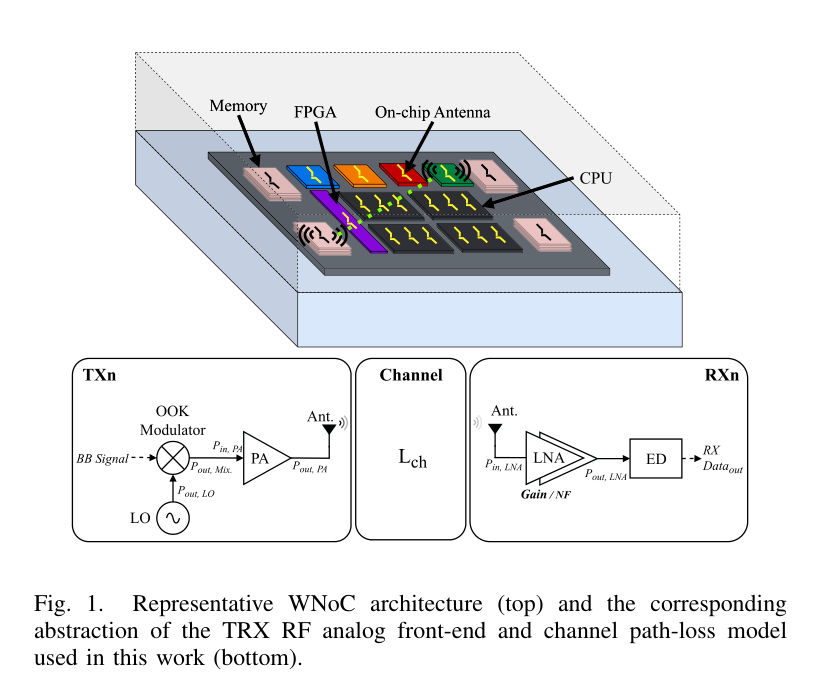
\includegraphics[width=0.88\textwidth]{chapters/ch10-optical-wireless/figures/shahmoradi_fig01_wnoc_architecture.png}
\caption{Wireless Network-on-Chip (WNoC) system architecture illustrating the integrated RF transceiver (TRX) front-end abstraction, on-chip planar antenna, and propagation channel through the lossy silicon/dielectric stack. [Reproduced from: M. Shahmoradi et al., ``Channel-Aware Behavioral Power Modeling of CMOS OOK Transceivers for Wireless Network-on-Chip Systems'', \emph{IEEE Transactions on Circuits and Systems I: Regular Papers}, Vol. 73, No. 4, pp. 1620--1633, 2026, DOI: 10.5281/zenodo.19449802.~\cite{Shahmoradi2026} \copyright\ 2026 IEEE]}
\label{fig:shahmoradi-wnoc-arch}
\end{figure}

\subsection{System Architecture \& Transceiver Front-End}

As formulated by Shahmoradi et al.~\cite{Shahmoradi2026} and illustrated in Fig.~\ref{fig:shahmoradi-wnoc-arch}, an on-chip wireless link consists of three sub-systems:
\begin{enumerate}
    \item \textbf{Transmitter (TX)}: Comprises a high-speed modulator, local voltage-controlled oscillator (VCO), and RF Power Amplifier (PA). Non-coherent \textbf{On-Off Keying (OOK)} is predominantly employed in WNoC designs because it avoids power-hungry phase-locked loops and carrier synchronization circuits.
    
    \item \textbf{Propagation Channel \& Integrated Antennas}: Planar dipole, zigzag, or patch antennas fabricated in top metal layers transmit through the multi-layer dielectric package. In standard bulk silicon, electromagnetic waves suffer high attenuation ($25\text{--}35\,\mathrm{dB}$) due to substrate conductivity ($\sigma_{\mathrm{Si}} \approx 10\,\mathrm{S/m}$), requiring high-resistivity silicon substrates ($\sigma < 0.1\,\mathrm{S/m}$) or silicon dioxide trenches to reduce path loss.
    
    \item \textbf{Receiver (RX)}: Consists of a Low-Noise Amplifier (LNA), an Envelope Detector (ED) for direct non-coherent downconversion, and a baseband limiting amplifier.
\end{enumerate}

\subsection{Channel-Aware Power Allocation \& Operating Frequencies}

\begin{figure}[htbp]
\centering
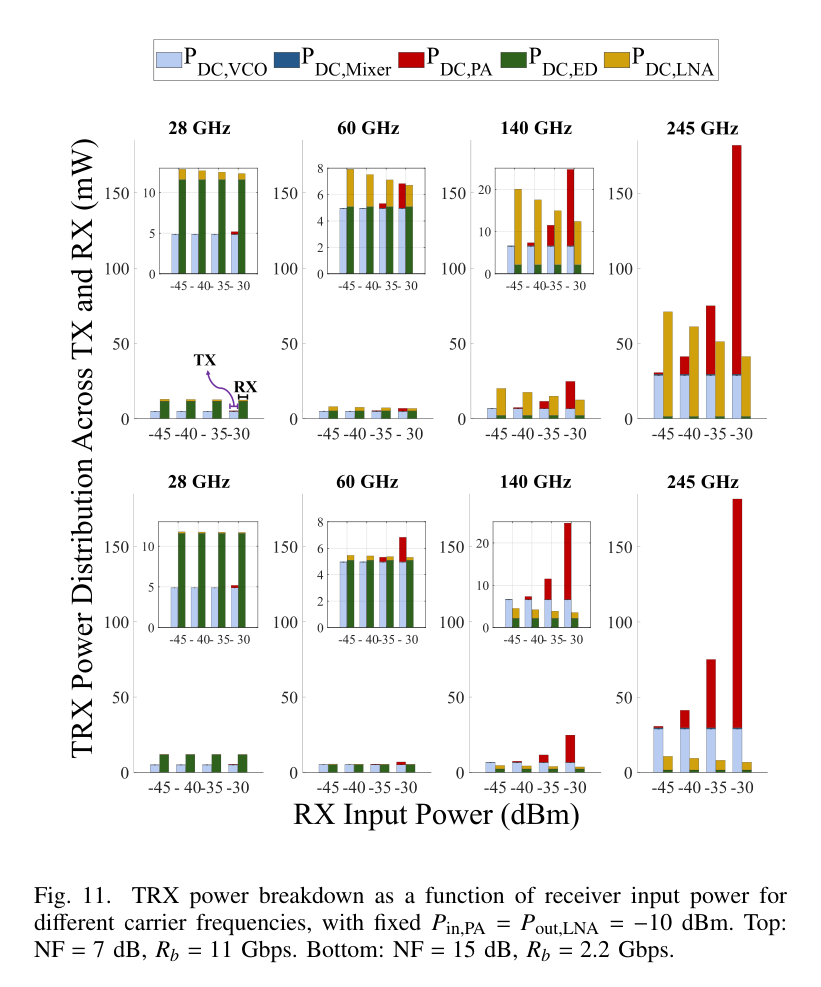
\includegraphics[width=0.88\textwidth]{chapters/ch10-optical-wireless/figures/shahmoradi_fig11_trx_power_optima.png}
\caption{Continuous contour maps of total RF transceiver power consumption versus carrier frequency and received power under stringent ($\mathrm{NF} = 7\,\mathrm{dB}$) and relaxed ($\mathrm{NF} = 15\,\mathrm{dB}$) receiver noise figures, highlighting optimal operating points across 28, 60, 140, and 245 GHz. [Reproduced from: M. Shahmoradi et al., ``Channel-Aware Behavioral Power Modeling of CMOS OOK Transceivers for Wireless Network-on-Chip Systems'', \emph{IEEE Transactions on Circuits and Systems I: Regular Papers}, Vol. 73, No. 4, pp. 1620--1633, 2026, DOI: 10.5281/zenodo.19449802.~\cite{Shahmoradi2026} \copyright\ 2026 IEEE]}
\label{fig:shahmoradi-power-optima}
\end{figure}

The total DC power consumption of the transceiver front-end is $P_{\mathrm{DC,TRX}} = P_{\mathrm{DC,TX}} + P_{\mathrm{DC,RX}}$. Fig.~\ref{fig:shahmoradi-power-optima} presents the continuous power optimization contours established by Shahmoradi et al.~\cite{Shahmoradi2026}. At lower frequencies ($28\text{--}60\,\mathrm{GHz}$), CMOS transistors operate well below their unity-current-gain cut-off frequency ($f_T$), achieving optimal energy efficiency around $60\,\mathrm{GHz}$ ($\approx 15\text{--}25\,\mathrm{mW}$ total TRX dissipation for $10\text{--}16\,\mathrm{Gbps}$ line rates). At sub-THz bands ($140\text{--}245\,\mathrm{GHz}$), antenna dimensions shrink below $500\,\mu\mathrm{m}$, enabling compact tile integration, but Power Amplifier efficiency degrades rapidly, increasing transmitter power demands.

\section{Hardware Implementation: Synthesizable Photonic MRR Switch}
\label{sec:photonic-verilog}

Listing~\ref{lst:photonic-mrr-verilog} presents the synthesizable Verilog implementation of an electro-optic Micro-Ring Resonator switching controller with closed-loop proportional thermal resonance tracking and pulse-width modulated (PWM) microheater actuation.

\begin{lstlisting}[language=Verilog, caption={Synthesizable Photonic MRR Switch Controller with Closed-Loop Thermal Tuning (\texttt{photonic\_mrr\_switch.v})}, label={lst:photonic-mrr-verilog}]
module photonic_mrr_switch #(
    parameter TEMP_WIDTH      = 10,      // 0.1 deg C LSB resolution
    parameter TARGET_TEMP     = 10'd550, // 55.0 deg C target resonance
    parameter PWM_WIDTH       = 8,       // 8-bit microheater DAC resolution
    parameter LOCK_TOLERANCE  = 10'd5    // +/- 0.5 deg C lock window
)(
    input  wire                   clk,
    input  wire                   rst_n,

    // Optical Switching Command Interface
    input  wire                   switch_cmd,    // 0 = Through, 1 = Drop
    output reg                    optical_state, // Actuated optical routing state
    output reg                    switch_ready,  // Asserted when resonance is locked

    // Digital Thermal Sensor Feedback
    input  wire [TEMP_WIDTH-1:0]  measured_temp,
    input  wire                   temp_valid,

    // Microheater Control Outputs
    output reg  [PWM_WIDTH-1:0]   heater_power_val,
    output wire                   heater_pwm_pulse,
    output reg                    thermal_alarm
);

    reg [PWM_WIDTH-1:0] pwm_counter;

    // PWM Pulse Generator for Resistive Microheater
    assign heater_pwm_pulse = (pwm_counter < heater_power_val);

    always @(posedge clk or negedge rst_n) begin
        if (!rst_n) pwm_counter <= {PWM_WIDTH{1'b0}};
        else        pwm_counter <= pwm_counter + 1'b1;
    end

    // Proportional Thermal Resonance Tracking Loop
    always @(posedge clk or negedge rst_n) begin
        if (!rst_n) begin
            heater_power_val <= 8'd128; // 50% initial duty cycle
            optical_state    <= 1'b0;
            switch_ready     <= 1'b0;
            thermal_alarm    <= 1'b0;
        end else begin
            if (temp_valid) begin
                if (measured_temp < TARGET_TEMP) begin
                    // Cavity cold: boost microheater actuation
                    if (heater_power_val < 8'd250)
                        heater_power_val <= heater_power_val + 8'd2;
                end else begin
                    // Cavity hot: reduce heater actuation
                    if (heater_power_val > 8'd5)
                        heater_power_val <= heater_power_val - 8'd2;
                end

                // Verify thermal locking within tolerance
                if ((measured_temp >= (TARGET_TEMP - LOCK_TOLERANCE)) &&
                    (measured_temp <= (TARGET_TEMP + LOCK_TOLERANCE))) begin
                    switch_ready  <= 1'b1;
                    thermal_alarm <= 1'b0;
                end else begin
                    switch_ready  <= 1'b0;
                    if (measured_temp > (TARGET_TEMP + 10'd200))
                        thermal_alarm <= 1'b1;
                    else
                        thermal_alarm <= 1'b0;
                end
            end

            // Optical routing actuation: default safe to Through state if unlocked
            if (switch_ready) optical_state <= switch_cmd;
            else              optical_state <= 1'b0;
        end
    end
endmodule
\end{lstlisting}

\section{Simulation Model \& Numerical Verification}
\label{sec:optical-sim-verification}

The Python model \texttt{onoc\_optical\_loss\_sim.py} simulates end-to-end insertion loss, laser power, and thermal tuning requirements across an $8 \times 8$ mesh ONoC (64 compute nodes, $20\,\mathrm{mm} \times 20\,\mathrm{mm}$ die area) comparing traditional Crossing Switching Elements (CSEs) against Parallel Switching Elements (PSEs). Table~\ref{tab:onoc-results} summarizes the experimental metrics.

\begin{table}[htbp]
\centering
\caption{Comparative Evaluation: Crossing Switching Elements (CSE) vs. Parallel Switching Elements (PSE) in an $8 \times 8$ ONoC}
\label{tab:onoc-results}
\begin{tabular}{lcc}
\hline
\textbf{Metric} & \textbf{CSE Architecture} & \textbf{PSE Architecture (Kao et al.)} \\
\hline
Waveguide Crossings & $62$ & $\mathbf{24}$ ($-61.3\%$) \\
Active MRR Count & $192$ & $\mathbf{112}$ ($-41.7\%$) \\
Worst-Case Insertion Loss & $11.38\,\mathrm{dB}$ & $\mathbf{6.38\,\mathrm{dB}}$ ($\mathbf{-5.00\,\mathrm{dB}}$) \\
Required Optical Laser Power & $0.27\,\mathrm{mW}$ & $\mathbf{0.09\,\mathrm{mW}}$ ($3.0\times\text{ lower}$) \\
Laser Electrical Wall-Plug Power & $1.37\,\mathrm{mW}$ & $\mathbf{0.43\,\mathrm{mW}}$ \\
Thermal Tuning Power ($15^\circ\mathrm{C}$ spread) & $5184.0\,\mathrm{mW}$ & $\mathbf{3024.0\,\mathrm{mW}}$ ($-41.7\%$) \\
Total Optical Subsystem Power & $5185.4\,\mathrm{mW}$ & $\mathbf{3024.4\,\mathrm{mW}}$ ($\mathbf{-41.7\%}$) \\
\hline
\end{tabular}
\end{table}

The simulation results confirm that by eliminating internal crossings, the PSE architecture reduces maximum insertion loss by $5.00\,\mathrm{dB}$. Because optical laser power scales exponentially with decibel loss, this $5\,\mathrm{dB}$ reduction cuts optical source power requirements by $3\times$. Furthermore, reducing MRR usage from 192 to 112 directly slashes active thermal tuning dissipation from $5.18\,\mathrm{W}$ to $3.02\,\mathrm{W}$, proving that physically aware topology synthesis is mandatory for practical optical networks.

\section{Summary}
\label{sec:ch10_summary}

Optical Networks-on-Chip (ONoC) and Wireless Networks-on-Chip (WNoC) transcend the physical limitations of metallic interconnects. Nanophotonics provides massive bandwidth density through WDM lightwaves propagating at the speed of light, while Parallel Switching Elements (PSEs) and Add-Drop Filters (ADFs) minimize crossing losses and laser power. Concurrently, mmWave wireless links provide single-hop broadcast capabilities that bypass multi-hop planar mesh delays. Overcoming thermal resonance drift in silicon resonators and managing RF transceiver front-end power efficiency represent the critical research frontiers for next-generation on-chip non-traditional fabrics.

\section{Exercises and Review Questions}
\label{sec:ch10_exercises}

\begin{enumerate}
    \item \textbf{Micro-Ring Resonator Resonance Calculation}: An on-chip silicon ring resonator has radius $R = 6.0\,\mu\mathrm{m}$ and an effective refractive index $n_{\mathrm{eff}} = 2.45$ at optical wavelength $\lambda_0 = 1550\,\mathrm{nm}$.
    \begin{enumerate}
        \item Calculate the optical round-trip cavity path length $L = 2 \pi R$.
        \item Determine the integer resonant mode order $m$.
        \item Compute the Free Spectral Range (FSR) of the resonator in nanometers, assuming group index $n_{\mathrm{g}} = 4.20$ ($\mathrm{FSR} = \lambda_0^2 / (n_{\mathrm{g}} L)$).
    \end{enumerate}

    \item \textbf{Optical Link Budget \& Laser Sizing}: An optical communication lightpath traverses $3.5\,\mathrm{cm}$ of waveguide ($\alpha_{\mathrm{prop}} = 0.25\,\mathrm{dB/cm}$), undergoes 16 bends ($\alpha_{\mathrm{bend}} = 0.005\,\mathrm{dB}$), crosses 30 perpendicular waveguides ($\alpha_{\mathrm{cross}} = 0.12\,\mathrm{dB}$), passes 20 unselected MRRs ($\alpha_{\mathrm{thru}} = 0.015\,\mathrm{dB}$), and drops through 2 active MRRs ($\alpha_{\mathrm{drop}} = 0.50\,\mathrm{dB}$). Modulator insertion loss is $1.5\,\mathrm{dB}$, and photodetector sensitivity is $-21.0\,\mathrm{dBm}$.
    \begin{enumerate}
        \item Calculate the total end-to-end insertion loss $L_{\mathrm{path}}$ in decibels.
        \item For a $3.0\,\mathrm{dB}$ operating margin, compute the required laser optical output power in $\mathrm{dBm}$ and in milliwatts.
        \item If laser wall-plug efficiency is $\eta_{\mathrm{wpe}} = 18\%$, calculate the total electrical power consumed by the laser.
    \end{enumerate}

    \item \textbf{Thermal Tuning Overhead}: A multi-core processor exhibits a die temperature spread of $\Delta T = 20^\circ\mathrm{C}$ between edge and hotspot regions. If each MRR shifts by $d\lambda / dT = 0.10\,\mathrm{nm/^\circ C}$ and microheaters consume $20.0\,\mathrm{mW/nm}$ to red-shift resonant wavelengths:
    \begin{enumerate}
        \item Calculate the total wavelength drift $\Delta \lambda$ in nanometers.
        \item Compute the thermal tuning power per resonator.
        \item For a network deploying 128 active MRRs, calculate the total thermal tuning power overhead.
    \end{enumerate}

    \item \textbf{Wireless NoC Friis Transmission Budget}: An on-chip $60\,\mathrm{GHz}$ wireless link has transmitter and receiver antenna gains of $G_{\mathrm{tx}} = G_{\mathrm{rx}} = -2\,\mathrm{dBi}$ operating over a distance of $d = 12\,\mathrm{mm}$ in an effective dielectric medium with $\epsilon_{\mathrm{eff}} = 3.8$.
    \begin{enumerate}
        \item Calculate the guided wavelength $\lambda = c / (f \sqrt{\epsilon_{\mathrm{eff}}})$.
        \item Using Friis' transmission formula in decibels, calculate the path loss $PL = 20 \log_{10}(4 \pi d / \lambda) - G_{\mathrm{tx}} - G_{\mathrm{rx}}$.
        \item Explain why on-chip wireless channels experience higher attenuation than free-space wireless propagation.
    \end{enumerate}
\end{enumerate}

